\documentclass{beamer}

\usepackage[T1]{fontenc}
\usepackage[utf8]{inputenc}
\usepackage{lmodern}
\usepackage{amsmath,amssymb,amsfonts}
\usepackage{physics}
\usepackage{bm}
\usepackage{mathtools}
\usepackage{quantikz}

\title{From the Quantum Phase estimation algorithm to the HHL and QAOA algorithms}
\author{Morten Hjorth-Jensen}
\date{FYS5419/9419: Week of April 7-11, 2026}

\begin{document}

%------------------------------------------------
\frame{\titlepage}

%------------------------------------------------
\begin{frame}{Outline}
\begin{enumerate}
\item Quantum Phase Estimation (QPE)
\item Connection to Hamiltonian simulation
\item Connection to Variational Quantum Eigensolvers (VQE)
\item Introducing the HHL algorithm
\end{enumerate}
See also separate jupyter-notebooks at \url{https://github.com/CompPhysics/QuantumComputingMachineLearning/tree/gh-pages/doc/pub/week11/ipynb/week11.ipynb}
\end{frame}


%================================================
\begin{frame}{Quantum Phase Estimation: Problem Statement, reminder from Lecture March 25}
Suppose \(U\) is a unitary operator and \(\ket{\psi}\) is one of its eigenstates:
\[
U\ket{\psi}=e^{2\pi i \phi}\ket{\psi},
\qquad 0\le \phi <1.
\]

The goal of Quantum Phase Estimation (QPE) is to estimate the phase \(\phi\).

Equivalently, QPE extracts the eigenvalue of \(U\) in phase form.
\end{frame}

%================================================
\begin{frame}{Why QPE Matters}
QPE is central because many physical problems can be mapped to eigenvalue estimation.

Examples:
\begin{itemize}
\item energy estimation in quantum chemistry,
\item eigenvalue problems in many-body physics,
\item Hamiltonian simulation,
\item Shor's algorithm and period finding.
\end{itemize}

If we can encode a Hamiltonian into a unitary, then QPE can extract its eigenvalues.
\end{frame}

%================================================
\begin{frame}{Registers Used in QPE}
QPE uses two registers:

\begin{itemize}
\item a control register of \(n\) qubits, initialized in \(\ket{0}^{\otimes n}\),
\item a system register, initialized in the eigenstate \(\ket{\psi}\).
\end{itemize}

So the initial state is
\[
\ket{0}^{\otimes n}\ket{\psi}.
\]

The control register stores the estimated phase bits.
\end{frame}

%================================================
\begin{frame}{Step 1: Create a Uniform Superposition}
Apply Hadamard gates to all control qubits:
\[
\ket{0}^{\otimes n}
\mapsto
\frac{1}{2^{n/2}}
\sum_{k=0}^{2^n-1}\ket{k}.
\]

So the total state becomes
\[
\frac{1}{2^{n/2}}
\sum_{k=0}^{2^n-1}
\ket{k}\ket{\psi}.
\]

This prepares the control register as a coherent superposition of all binary numbers \(k\).
\end{frame}

%================================================
\begin{frame}{Step 2: Controlled Powers of \(U\)}
Now apply controlled powers of \(U\):
\[
U^{2^0}, U^{2^1}, U^{2^2}, \dots, U^{2^{n-1}}.
\]

Each control qubit determines whether the corresponding power is applied.

Because \(\ket{\psi}\) is an eigenstate,
\[
U^{2^j}\ket{\psi} = e^{2\pi i 2^j \phi}\ket{\psi}.
\]

Hence each controlled unitary writes phase information into the control register.
\end{frame}

%================================================
\begin{frame}{Step 2: State After Controlled Powers}
If the control register basis state is \(\ket{k}\), then the controlled operations apply \(U^k\), giving
\[
U^k\ket{\psi} = e^{2\pi i k\phi}\ket{\psi}.
\]

Therefore the combined state becomes
\[
\frac{1}{2^{n/2}}
\sum_{k=0}^{2^n-1}
e^{2\pi i k\phi}\ket{k}\ket{\psi}.
\]

The system register factors out, and the control register now contains the phase information.
\end{frame}

%================================================
\begin{frame}{Key Observation}
The control register is in the state
\[
\frac{1}{2^{n/2}}
\sum_{k=0}^{2^n-1} e^{2\pi i k\phi}\ket{k},
\]
which is exactly a Fourier-type state.

This is why the inverse QFT is the correct next step:
it converts this phase-encoded superposition into a computational basis approximation of \(\phi\).
\end{frame}

%================================================
\begin{frame}{Step 3: Apply the Inverse QFT}
Applying \(\mathrm{QFT}^{-1}\) to the control register gives
\[
\mathrm{QFT}^{-1}
\left(
\frac{1}{2^{n/2}}
\sum_{k=0}^{2^n-1} e^{2\pi i k\phi}\ket{k}
\right).
\]

If
\[
\phi = \frac{m}{2^n}
\]
exactly for some integer \(m\), then this becomes
\[
\ket{m}.
\]

So the control register stores the exact \(n\)-bit binary expansion of \(\phi\).
\end{frame}

%================================================
\begin{frame}{Exact QPE Case}
Suppose
\[
\phi = 0.\phi_1\phi_2\dots\phi_n
=
\frac{m}{2^n}.
\]

Then after inverse QFT, the control register becomes
\[
\ket{\phi_1\phi_2\dots\phi_n}.
\]

Thus measuring the control register returns the exact binary digits of \(\phi\).

This is the cleanest case of QPE.
\end{frame}

%================================================
\begin{frame}{Step-by-Step Derivation with Binary Fractions}
Let
\[
\phi = 0.\phi_1\phi_2\dots\phi_n\dots
\]

Then one can show that the control-register state after controlled powers factorizes as
\[
\frac{1}{2^{n/2}}
\left(\ket0 + e^{2\pi i\, 2^{n-1}\phi}\ket1\right)
\otimes
\left(\ket0 + e^{2\pi i\, 2^{n-2}\phi}\ket1\right)
\otimes \cdots
\]
\[
\cdots \otimes
\left(\ket0 + e^{2\pi i\, \phi}\ket1\right).
\]

Because
\[
2^{n-1}\phi = \phi_1.\phi_2\phi_3\dots,
\]
only the fractional parts matter in the phases, so each qubit encodes one successive binary suffix.
\end{frame}

%================================================
\begin{frame}{How the Bits Emerge}
Using the binary expansion of \(\phi\), the control-register state becomes
\[
\frac{1}{2^{n/2}}
\left(\ket0 + e^{2\pi i\,0.\phi_n}\ket1\right)
\otimes
\left(\ket0 + e^{2\pi i\,0.\phi_{n-1}\phi_n}\ket1\right)
\otimes \cdots
\]
\[
\cdots \otimes
\left(\ket0 + e^{2\pi i\,0.\phi_1\phi_2\dots\phi_n}\ket1\right),
\]
which has exactly the structure of a QFT state.

Therefore applying \(\mathrm{QFT}^{-1}\) yields the bit string
\[
\phi_1\phi_2\dots\phi_n.
\]
\end{frame}

%================================================
\begin{frame}{QPE Circuit}
\centering
\begin{quantikz}
\lstick{$\ket{0}$}    & \gate{H} & \ctrl{3} & \qw      & \qw      & \gate[3]{\mathrm{QFT}^\dagger} & \meter{} \\
\lstick{$\ket{0}$}    & \gate{H} & \qw      & \ctrl{2} & \qw      & \ghost{\mathrm{QFT}^\dagger}   & \meter{} \\
\lstick{$\ket{0}$}    & \gate{H} & \qw      & \qw      & \ctrl{1} & \ghost{\mathrm{QFT}^\dagger}   & \meter{} \\
\lstick{$\ket{\psi}$} & \qw      & \gate{U^4} & \gate{U^2} & \gate{U} & \qw                          & \qw
\end{quantikz}

\vspace{0.5em}

This example shows a 3-qubit control register and one system register.
\end{frame}

%================================================
\begin{frame}{Worked Example: \(\phi=5/8\)}
Suppose
\[
\phi = \frac{5}{8} = 0.101.
\]

Then the ideal QPE output on a 3-qubit control register is
\[
\ket{101}.
\]

Indeed,
\[
e^{2\pi i \phi} = e^{2\pi i (5/8)}.
\]

After the controlled powers and inverse QFT, the control register collapses to the bit string \(101\) with probability 1.
\end{frame}

%================================================
\begin{frame}{When \(\phi\) Is Not Exactly Representable}
If \(\phi\) is not exactly of the form \(m/2^n\), then QPE does not return one exact bit string.

Instead, the output is a probability distribution peaked near the best \(n\)-bit approximation:
\[
\phi \approx \frac{m}{2^n}.
\]

The measurement outcome gives the nearest binary approximation with high probability.
\end{frame}

%================================================
\begin{frame}{Precision of QPE}
With \(n\) control qubits, QPE resolves phases to approximately
\[
\Delta \phi \sim \frac{1}{2^n}.
\]

Thus the precision improves exponentially with the number of control qubits.

This exponential precision is one of the main reasons QPE is so powerful.
\end{frame}

%================================================
\begin{frame}{From Phases to Energies}
Suppose \(H\) is a Hamiltonian with eigenstate \(\ket{E}\):
\[
H\ket{E} = E\ket{E}.
\]

Define the time-evolution operator
\[
U(t)=e^{-iHt}.
\]

Then
\[
U(t)\ket{E} = e^{-iEt}\ket{E}.
\]

Comparing with
\[
U\ket{\psi}=e^{2\pi i \phi}\ket{\psi},
\]
we identify
\[
\phi = -\frac{Et}{2\pi} \mod 1.
\]

Thus QPE can estimate energies if we can implement \(e^{-iHt}\).
\end{frame}

%================================================
\begin{frame}{Connection to Hamiltonian Simulation}
QPE requires controlled applications of
\[
U^{2^j} = e^{-iH t 2^j}.
\]

So QPE depends directly on the ability to perform Hamiltonian simulation.

In practice this may be done using:
\begin{itemize}
\item Trotter-Suzuki decompositions,
\item linear-combination-of-unitaries methods,
\item qubitization,
\item problem-specific simulation techniques.
\end{itemize}

Thus:
\[
\text{Hamiltonian simulation} + \text{QPE}
\quad \Rightarrow \quad
\text{energy estimation}.
\]
\end{frame}

%================================================
\begin{frame}{Physical Interpretation}
QPE measures the dynamical phase accumulated by an energy eigenstate under time evolution.

The algorithm turns the phase
\[
e^{-iEt}
\]
into a bit string encoding the energy.

So one can view QPE as a highly precise interferometric energy-measurement protocol.
\end{frame}

%================================================
\begin{frame}{Why QPE Is Important in Quantum Chemistry}
In quantum chemistry and many-body physics, the main goal is often to compute eigenenergies of a Hamiltonian.

If we can prepare an approximate eigenstate with sufficient overlap with the true ground state, then QPE can project onto the exact eigenvalue with high precision.

This makes QPE a natural route to:
\begin{itemize}
\item ground-state energies,
\item excited-state energies,
\item spectral properties.
\end{itemize}
\end{frame}

%================================================
\begin{frame}{Connection to VQE}
The Variational Quantum Eigensolver (VQE) and QPE aim at similar physics goals, but in different ways.

\textbf{VQE:}
\begin{itemize}
\item variational,
\item hybrid quantum-classical,
\item optimized by minimizing
\[
E(\bm{\theta}) = \bra{\psi(\bm{\theta})} H \ket{\psi(\bm{\theta})},
\]
\item suitable for noisy near-term devices.
\end{itemize}

\textbf{QPE:}
\begin{itemize}
\item not variational,
\item requires coherent controlled time evolution,
\item provides direct eigenvalue estimation,
\item suited to fault-tolerant quantum computers.
\end{itemize}
\end{frame}

%================================================
\begin{frame}{How VQE and QPE Complement Each Other}
A common long-term strategy is:
\begin{enumerate}
\item Use a variational method such as VQE to prepare a good approximate eigenstate
\[
\ket{\psi_{\mathrm{trial}}}
\]
with large overlap with the true eigenstate.

\item Use that state as the input to QPE.

\item QPE then refines the energy estimate to high precision.
\end{enumerate}

So VQE can be viewed as a state-preparation front end for QPE.
\end{frame}

%================================================
\begin{frame}{Overlap Requirement}
If the initial state is
\[
\ket{\psi_{\mathrm{trial}}} = \sum_j c_j \ket{E_j},
\]
then QPE outputs \(E_j\) with probability
\[
|c_j|^2.
\]

Therefore the success probability depends on the overlap with the desired eigenstate.

This is exactly why improved ans\"atze in VQE are also valuable for QPE-based workflows.
\end{frame}

%================================================
\begin{frame}{QPE vs VQE in Practice}
\textbf{VQE}
\begin{itemize}
\item shallow circuits,
\item many repeated measurements,
\item classical optimization loop,
\item noise tolerant,
\item limited by optimization difficulty and shot cost.
\end{itemize}

\textbf{QPE}
\begin{itemize}
\item deep coherent circuits,
\item requires controlled \(e^{-iHt}\),
\item very precise,
\item ideal for fault-tolerant hardware,
\item often viewed as the long-term gold standard for energy estimation.
\end{itemize}
\end{frame}

%================================================
\begin{frame}{Semiclassical Interpretation}
One may interpret QPE as repeatedly extracting successive binary digits of a phase.

The inverse QFT acts globally, but conceptually it decodes the phase one bit at a time.

This bitwise structure is one reason QPE is so elegant mathematically.
\end{frame}

%================================================
\begin{frame}{Implementation}
A implementation of the QPE typically proceeds as follows:
\begin{enumerate}
\item choose the number of control qubits,
\item initialize the system register in an eigenstate or approximate eigenstate,
\item apply Hadamards to the control register,
\item apply controlled \(U^{2^j}\),
\item apply inverse QFT,
\item measure the control register,
\item interpret the measurement as an estimate of \(\phi\).
\end{enumerate}

If the notebook also implements the QFT explicitly, it will usually reuse the same Hadamard + controlled-phase + swap pattern.
\end{frame}

%================================================
\begin{frame}{Summary of the Full Picture}
\[
\text{Hamiltonian } H
\quad \longrightarrow \quad
U(t)=e^{-iHt}
\quad \longrightarrow \quad
\text{QPE}
\quad \longrightarrow \quad
E
\]

The QFT is the phase-decoding engine inside QPE.

VQE and QPE are complementary:
\begin{itemize}
\item VQE is a near-term variational energy estimator,
\item QPE is a long-term high-precision eigenvalue estimator,
\item VQE can provide input states for QPE.
\end{itemize}
\end{frame}

%================================================
\begin{frame}{Summary}
We have seen that:
\begin{itemize}
\item the QFT maps
\[
\ket{x}\mapsto \frac{1}{\sqrt N}\sum_k e^{2\pi i xk/N}\ket{k},
\]
\item QPE uses controlled powers of a unitary and the inverse QFT to extract eigenphases,
\item for Hamiltonian evolution
\[
U(t)=e^{-iHt},
\]
QPE becomes an energy-estimation algorithm,
\item VQE and QPE address related eigenvalue problems with different hardware requirements.
\end{itemize}
\end{frame}

%================================================
\begin{frame}{Suggestions for the second project}
\begin{itemize}
\item Continuation of project 1 with  more realistic systems and using adaptive VQE on actual (real) quantum computers
\item Implementation and studies of the Quantum Approximate Optimization Algorithm (QAOA): Simulation of linear algebra systems on quantum computers, solving for example differential equations
\item Implementation of the HHL algorithm (needs QPE)
\item Applications and implementations of quantum machine learning algorithms
\item Implement quantum neural networks for PINNs
\item Detailed quantum chemistry applications.
\end{itemize}
\end{frame}



\begin{frame}{Suggestions for the second project}
\begin{itemize}
\item Studies of entanglement and physical realization of quantum gates and circuits
\item Implementing Shor's algorithm or other algorithms
\item Parallelizing the Variational Quantum Eigensolver with multi-GPU scaling, see \url{https://arxiv.org/abs/2601.09951}
\item Implementing and comparing the quantum phase estimation algorithm with VQE, see for example recent QPE paper at \url{"https://arxiv.org/abs/2601.05788}
\item Studies of hyperparameters in VQE, see for example \url{https://arxiv.org/abs/2601.16679}
\item Implementing unitary coupled cluster theory on a quantum computer, see \url{https://arxiv.org/abs/2501.15893}
\end{itemize}
\end{frame}


\begin{frame}{What is the HHL algorithm?}

The HHL algorithm—named after Aram Harrow, Avinatan Hassidim, and Seth
Lloyd—is one of the central quantum algorithms for solving linear
systems of equations.

The core idea is to solve a linear system
\[
A \mathbf{x} = \mathbf{b}.
\]
\end{frame}

\begin{frame}{What is the QAOA algorithm?, to be discussed April 15}
\begin{block}{QAOA stands for the Quantum Approximate Optimization Algorithm}
Each part of the name reflects something essential about the method:
\begin{itemize}
\item Quantum: it runs on a quantum computer, using qubits and quantum gates.
\item Approximate: it typically finds near-optimal solutions rather than exact ones.
\item Optimization: it is designed to solve optimization problems (like MaxCut, scheduling, portfolio selection).
\item Algorithm: it is a well-defined hybrid quantum–classical procedure.
\end{itemize}
\end{block}

QAOA is a variational quantum algorithm that uses a parameterized quantum circuit to search for good solutions to hard optimization problems.
\end{frame}


\begin{frame}{HHL: Linear Systems Everywhere}
\begin{itemize}
\item Solve:
\[
A \mathbf{x} = \mathbf{b}
\]
\item Appears in:
\begin{itemize}
\item PDEs
\item Machine learning
\item Many-body physics
\end{itemize}
\item Classical cost: $\mathcal{O}(N^3)$ (dense case)
\end{itemize}
\end{frame}

%------------------------------------------------

\begin{frame}{Quantum Goal}
\begin{itemize}
\item Encode vector as quantum state:
\[
|b\rangle = \sum_i b_i |i\rangle
\]
\item Goal:
\[
|x\rangle \propto A^{-1}|b\rangle
\]
\item Output is a quantum state, not a classical vector
\end{itemize}
\end{frame}


\begin{frame}{Eigenbasis Representation}
\[
A |u_j\rangle = \lambda_j |u_j\rangle
\]
\[
|b\rangle = \sum_j \beta_j |u_j\rangle
\]
\end{frame}

%------------------------------------------------

\begin{frame}{Formal Solution}
\[
A^{-1}|b\rangle = \sum_j \frac{\beta_j}{\lambda_j} |u_j\rangle
\]
\begin{itemize}
\item Problem reduces to eigenvalue inversion
\end{itemize}
\end{frame}



\begin{frame}{Hamiltonian Encoding}
\begin{itemize}
\item Assume $A$ is Hermitian
\item Implement:
\[
U = e^{iAt}
\]
\end{itemize}
\end{frame}

%------------------------------------------------

\begin{frame}{QPE Action}
\[
|u_j\rangle \rightarrow |u_j\rangle |\lambda_j\rangle
\]
\end{frame}

%------------------------------------------------

\begin{frame}{State After QPE}
\[
\sum_j \beta_j |u_j\rangle |\lambda_j\rangle
\]
\end{frame}


\begin{frame}{Key Step: Inversion}
\begin{itemize}
\item Introduce ancilla qubit
\item Perform controlled rotation:
\[
|\lambda_j\rangle \rightarrow
\sqrt{1-\frac{C^2}{\lambda_j^2}}|0\rangle +
\frac{C}{\lambda_j}|1\rangle
\]
\end{itemize}
\end{frame}

%------------------------------------------------

\begin{frame}{State After Rotation}
\[
\sum_j \beta_j |u_j\rangle |\lambda_j\rangle
\left(
\sqrt{1-\frac{C^2}{\lambda_j^2}}|0\rangle +
\frac{C}{\lambda_j}|1\rangle
\right)
\]
\end{frame}



\begin{frame}{Inverse QPE}
\begin{itemize}
\item Remove eigenvalue register
\item Leaves:
\[
\sum_j \frac{\beta_j}{\lambda_j}|u_j\rangle
\]
\end{itemize}
\end{frame}

%------------------------------------------------

\begin{frame}{Final State}
\[
|x\rangle \propto A^{-1}|b\rangle
\]
\end{frame}



\begin{frame}{HHL Circuit (Overview)}
\centering
\begin{quantikz}
\lstick{$|b\rangle$} & \qw & \qw & \qw & \qw & \qw \\
\lstick{$|0\rangle^{\otimes m}$} & \gate{QPE} & \qw & \gate{QPE^\dagger} & \qw & \qw \\
\lstick{$|0\rangle$} & \qw & \gate{R(\lambda^{-1})} & \qw & \meter{} & \qw
\end{quantikz}
\end{frame}


\begin{frame}{Detailed Circuit Step 1: QPE}
\centering
\begin{quantikz}
\lstick{$|b\rangle$} & \ctrl{1} & \qw \\
\lstick{$|0\rangle$} & \gate{e^{iAt}} & \qw
\end{quantikz}
\end{frame}

%------------------------------------------------

\begin{frame}{Detailed Circuit Step 2: Controlled Rotation}
\centering
\begin{quantikz}
\lstick{$|\lambda\rangle$} & \ctrl{1} & \qw \\
\lstick{$|0\rangle$} & \gate{R_y(\lambda^{-1})} & \qw
\end{quantikz}
\end{frame}

%------------------------------------------------

\begin{frame}{Detailed Circuit Step 3: Uncomputation}
\centering
\begin{quantikz}
\lstick{} & \gate{QPE^\dagger} & \qw
\end{quantikz}
\end{frame}



\begin{frame}{Post-selection and measurement}
\begin{itemize}
\item Measure ancilla
\item Condition on $|1\rangle$
\item Success probability depends on $\kappa$
\end{itemize}
\end{frame}


\begin{frame}{Runtime}
\[
\mathcal{O}\left(\kappa^2 \log N\right)
\]
\begin{itemize}
\item $\kappa$ = condition number
\end{itemize}
\end{frame}


\begin{frame}{Conditions for Speedup}
\begin{itemize}
\item Sparse matrix
\item Efficient Hamiltonian simulation
\item Efficient state preparation
\end{itemize}
\end{frame}


\begin{frame}{Readout Problem}
\begin{itemize}
\item Cannot extract full vector efficiently
\item Only expectation values accessible
\end{itemize}
\end{frame}

%------------------------------------------------

\begin{frame}{Condition Number Issue}
\begin{itemize}
\item Runtime scales with $\kappa$
\item Ill-conditioned systems are hard
\end{itemize}
\end{frame}


\begin{frame}{Operator View}
\[
A^{-1} = \sum_j \frac{1}{\lambda_j} |u_j\rangle \langle u_j|
\]
\end{frame}

%------------------------------------------------

\begin{frame}{Connection to Green's Functions}
\[
G = (A)^{-1}
\]
\begin{itemize}
\item Resolvent operator
\item Linear response theory
\end{itemize}
\end{frame}

%------------------------------------------------

\begin{frame}{Many-Body Perspective}
\begin{itemize}
\item HHL = spectral filtering
\item Similar to:
\begin{itemize}
\item Imaginary time evolution
\item Projection methods
\end{itemize}
\end{itemize}
\end{frame}


\begin{frame}{Applications}
\begin{itemize}
\item Quantum machine learning
\item PDE solvers
\item Data fitting
\end{itemize}
\end{frame}



\begin{frame}{Summary HHL}
\begin{itemize}
\item HHL solves $A x = b$ in quantum form
\item Uses:
\begin{itemize}
\item Phase estimation
\item Controlled rotation
\item Uncomputation
\end{itemize}
\item Connects strongly to spectral physics
\end{itemize}
\end{frame}



\begin{frame}{From Linear Systems to Resolvents, HHL and Green's function theory}
A central observation is that HHL solves a linear system
\[
A x = b
\]
by preparing a quantum state proportional to
\[
|x\rangle \propto A^{-1}|b\rangle.
\]
In many-body physics, the inverse of an operator is precisely the basic structure of a
\emph{resolvent} or \emph{Green's function}.

If we define
\[
G(z) = (z I - H)^{-1},
\]
then solving
\[
(zI-H)|x\rangle = |b\rangle
\]
is equivalent to preparing
\[
|x\rangle = G(z)|b\rangle.
\]

Thus HHL may be viewed as a quantum algorithm for applying a resolvent operator to a source state.
\end{frame}

%------------------------------------------------

\begin{frame}{Spectral Form of the Green's Function}
Let
\[
H|u_j\rangle = E_j |u_j\rangle.
\]
Then the resolvent has the spectral decomposition
\[
G(z) = (zI-H)^{-1}
= \sum_j \frac{1}{z-E_j} |u_j\rangle \langle u_j|.
\]
If
\[
|b\rangle = \sum_j \beta_j |u_j\rangle,
\]
then
\[
G(z)|b\rangle = \sum_j \frac{\beta_j}{z-E_j}|u_j\rangle.
\]

This is structurally identical to the HHL transformation:
\[
A^{-1}|b\rangle
=
\sum_j \frac{\beta_j}{\lambda_j}|u_j\rangle.
\]

Hence, HHL implements the same spectral inversion mechanism that underlies Green's functions.
\end{frame}

%------------------------------------------------~
\begin{frame}{Physical Meaning of the Spectral Filter}
  The factor
  \[
  \frac{1}{z-E_j}
  \]
  acts as a spectral filter.

  \begin{itemize}
  \item Eigenmodes with energies near \(z\) are enhanced.
  \item Eigenmodes far from \(z\) are suppressed.
  \item The inverse operator encodes propagation and response properties.
  \end{itemize}

  In this sense, HHL is not merely a linear solver. It is a \emph{spectral transformation algorithm}:
  it maps a source state to a response state through an inverse operator.
\end{frame}

%------------------------------------------------

\begin{frame}{Retarded Green's Function}
  In condensed matter and many-body theory, one often uses
  \[
  G^R(\omega) = \frac{1}{\omega + i\eta - H},
  \qquad \eta > 0.
  \]
  The small positive \(\eta\) regularizes the inverse and enforces causal boundary conditions.

  Applying this operator to a source state gives
  \[
  |x(\omega)\rangle = G^R(\omega)|b\rangle.
  \]

  Formally, an HHL-type algorithm can be interpreted as a way of preparing a quantum state proportional to this frequency-dependent response vector, provided one can encode the shifted operator
  \[
  A(\omega) = \omega I - H
  \]
  or
  \[
  A(\omega) = \omega I + i\eta - H.
  \]
\end{frame}

%------------------------------------------------

\begin{frame}{Connection to Correlation Functions}
  Many observables in quantum many-body physics can be written in terms of Green's functions or resolvents.

  For an operator \(\hat{O}\), a typical linear-response quantity has the form
  \[
  \chi(\omega)
  =
  \langle \psi_0 |
  \hat{O}^\dagger
  \frac{1}{\omega + i\eta - (H-E_0)}
  \hat{O}
  |\psi_0\rangle.
  \]
  If we define the source state
  \[
  |b\rangle = \hat{O}|\psi_0\rangle,
  \]
  then
  \[
  \chi(\omega)
  =
  \langle b|
  \frac{1}{\omega + i\eta - (H-E_0)}
  |b\rangle.
  \]

  This shows that HHL-like inversion is directly connected to computing dynamical susceptibilities.
\end{frame}

%------------------------------------------------

\begin{frame}{HHL as a Green's Function Engine}
  At a conceptual level, HHL performs three tasks:
  \begin{enumerate}
  \item Decompose the source state into eigenmodes.
  \item Invert the spectral coefficients:
    \[
    \lambda_j \mapsto \frac{1}{\lambda_j}.
    \]
  \item Recombine the filtered eigenmodes into the response state.
  \end{enumerate}

  This is exactly what is needed for:
  \begin{itemize}
  \item resolvent methods,
  \item Green's function methods,
  \item frequency-domain linear response,
  \item projection-based many-body calculations.
  \end{itemize}
\end{frame}


\begin{frame}{Linear Response in Physics}
  Suppose a system with Hamiltonian \(H_0\) is perturbed by
  \[
  V(t) = - f(t)\hat{F}.
  \]
  To first order, the expectation value of an observable \(\hat{O}\) changes as
  \[
  \delta \langle \hat{O}(t) \rangle
  =
  \int dt' \, \chi_{OF}(t-t') f(t'),
  \]
  where \(\chi_{OF}\) is the response function.

  In the frequency domain, one typically writes
  \[
  \delta \langle \hat{O}(\omega)\rangle
  =
  \chi_{OF}(\omega) f(\omega).
  \]

  The response function is often expressible through inverse operators of the form
  \[
  (\omega I - M)^{-1},
  \]
  which is precisely the structure targeted by HHL.
\end{frame}

%------------------------------------------------

\begin{frame}{Resolvent Form of the Susceptibility}
  A standard spectral representation is
  \[
  \chi_{OF}(\omega)
  =
  \sum_{n\neq 0}
  \left(
  \frac{\langle 0|\hat{O}|n\rangle \langle n|\hat{F}|0\rangle}
       {\omega-(E_n-E_0)+i\eta}
       -
       \frac{\langle 0|\hat{F}|n\rangle \langle n|\hat{O}|0\rangle}
            {\omega+(E_n-E_0)+i\eta}
            \right).
            \]
            This is a sum over poles, or equivalently a matrix element of a resolvent.

            Thus linear response is fundamentally an \emph{inverse-operator problem}, which places it in the same mathematical class as HHL.
\end{frame}



\begin{frame}{What is Time-Dependent Hartree--Fock?}
  Time-dependent Hartree--Fock (TDHF) describes the evolution of a Slater determinant under a time-dependent mean field.

  At the one-body density-matrix level,
  \[
  i\hbar \frac{d\rho}{dt} = [h[\rho],\rho].
  \]

  To study small oscillations around a stationary solution \(\rho_0\), one linearizes:
  \[
  \rho(t) = \rho_0 + \delta\rho(t),
  \]
  leading to an equation of motion for the fluctuation \(\delta\rho\).
\end{frame}

%------------------------------------------------

\begin{frame}{Linearized TDHF}
  After linearization, one obtains a matrix equation of the form
  \[
  i\hbar \frac{d}{dt}\delta \rho = \mathcal{L}\,\delta \rho + s(t),
  \]
  where:
  \begin{itemize}
  \item \(\mathcal{L}\) is the linearized Liouvillian or RPA matrix,
  \item \(s(t)\) is an external driving term.
  \end{itemize}

  In the frequency domain, this becomes
  \[
  (\omega I - \mathcal{L}) \delta \rho(\omega) = s(\omega).
  \]

  This is now explicitly a linear system. Its solution is
  \[
  \delta \rho(\omega) = (\omega I - \mathcal{L})^{-1} s(\omega).
  \]

  That is exactly the algebraic structure addressed by HHL.
\end{frame}

%------------------------------------------------

\begin{frame}{TDHF as an HHL-Type Problem}
  The formal similarity is immediate:
  \[
  A x = b
  \qquad \Longleftrightarrow \qquad
  (\omega I - \mathcal{L}) \delta \rho(\omega) = s(\omega).
  \]
  Hence:
  \[
  A \leftrightarrow \omega I - \mathcal{L},
  \qquad
  x \leftrightarrow \delta \rho(\omega),
  \qquad
  b \leftrightarrow s(\omega).
  \]

  If one can encode the linear-response matrix \(\mathcal{L}\) into a quantum representation, then an HHL-type algorithm could in principle prepare a state proportional to the TDHF response.
\end{frame}

%------------------------------------------------

\begin{frame}{Connection to Random Phase Approximation (RPA)}
  The small-amplitude limit of TDHF is closely related to the Random Phase Approximation (RPA).

  One typically obtains a non-Hermitian eigenvalue problem of the form
  \[
  \begin{pmatrix}
    A & B \\
    -B^* & -A^*
  \end{pmatrix}
  \begin{pmatrix}
    X \\ Y
  \end{pmatrix}
  =
  \omega
  \begin{pmatrix}
    X \\ Y
  \end{pmatrix}.
  \]
  Equivalently, one can formulate a driven linear-response problem
  \[
  (\omega I - M)\,v = s.
  \]

  Again, this is an inverse problem. The response amplitudes are obtained by applying the resolvent
  \[
  (\omega I - M)^{-1}
  \]
  to a source vector.
\end{frame}

%------------------------------------------------

\begin{frame}{What HHL Would Compute in TDHF}
  In a TDHF or RPA context, one is often interested in:
  \begin{itemize}
  \item transition amplitudes,
  \item density oscillations,
  \item response to an external field,
  \item strength functions.
  \end{itemize}

  These quantities can often be expressed as matrix elements involving the response vector:
  \[
  S(\omega) \sim \langle s | (\omega I - M)^{-1} | s \rangle.
  \]

  Thus an HHL-type routine would not need to output the full vector \(\delta\rho(\omega)\). It would already be useful if it allowed efficient estimation of such expectation values.
\end{frame}

%------------------------------------------------

\begin{frame}{Strength Functions and Dynamical Response}
  A common observable in TDHF and RPA is the strength function
  \[
  S_F(\omega)
  =
  -\frac{1}{\pi}\operatorname{Im}\chi_F(\omega),
  \]
  where
  \[
  \chi_F(\omega)
  =
  \langle 0|\hat{F}^\dagger
  \frac{1}{\omega + i\eta - (H-E_0)}
  \hat{F}|0\rangle.
  \]

  This is exactly a Green's function expression. Hence:
  \[
  \text{TDHF/RPA response}
  \quad \longleftrightarrow \quad
  \text{resolvent evaluation}
  \quad \longleftrightarrow \quad
  \text{HHL-type inversion}.
  \]
\end{frame}

%------------------------------------------------

\begin{frame}{Why This Connection is Interesting}
  The HHL framework is potentially relevant because:
  \begin{itemize}
  \item linear response is naturally formulated as a linear system,
  \item inverse operators define propagators and susceptibilities,
  \item many observables are expectation values rather than full vectors,
  \item this aligns well with quantum output models.
  \end{itemize}

  From a physics viewpoint, HHL is best interpreted not only as a solver of \(Ax=b\), but as a quantum method for preparing \emph{response states} and probing \emph{spectral properties}.
\end{frame}

%------------------------------------------------

\begin{frame}{Important Caveats}
  There are, however, important obstacles:
  \begin{itemize}
  \item The matrix \(A\) must be efficiently block-encoded or simulated.
  \item TDHF/RPA matrices may be non-Hermitian.
  \item Condition numbers may be large near resonances.
  \item State preparation and measurement may dominate the cost.
  \end{itemize}

  Therefore, the connection is mathematically deep and physically appealing, but practical advantage depends strongly on encoding, sparsity, conditioning, and the observables of interest.
\end{frame}

%------------------------------------------------

\begin{frame}{Hermitian Embedding of Non-Hermitian Problems}
  If the response matrix \(M\) is non-Hermitian, one common strategy is Hermitian embedding:
  \[
  \mathcal{H}
  =
  \begin{pmatrix}
    0 & M \\
    M^\dagger & 0
  \end{pmatrix}.
  \]
  Then \(\mathcal{H}\) is Hermitian, and one may reformulate the problem in an enlarged space.

  This is often the natural bridge between:
  \begin{itemize}
  \item non-Hermitian response equations,
  \item quantum phase estimation or HHL-type methods,
  \item Green's function formulations on quantum hardware.
  \end{itemize}
\end{frame}

%------------------------------------------------

\begin{frame}{Conceptual Summary}
  \begin{block}{Key idea}
    HHL applies an inverse operator spectrally:
    \[
    A^{-1} = \sum_j \frac{1}{\lambda_j}|u_j\rangle\langle u_j|.
    \]
  \end{block}

  \begin{block}{Green's function viewpoint}
    Choose
    \[
    A = zI - H,
    \]
    then HHL prepares a state proportional to
    \[
    (zI-H)^{-1}|b\rangle.
    \]
  \end{block}

  \begin{block}{TDHF / linear-response viewpoint}
    Choose
    \[
    A = \omega I - \mathcal{L},
    \]
    then HHL prepares a state proportional to the driven response
    \[
    \delta\rho(\omega) = (\omega I - \mathcal{L})^{-1} s(\omega).
    \]
  \end{block}
  \end{frame}




\begin{frame}{Linear Systems in Physics}
Many physics problems reduce to
\[
A x = b.
\]

Examples:
\begin{itemize}
\item discretized Schr\"odinger and diffusion equations,
\item linear response theory,
\item Green's function methods,
\item time-dependent Hartree--Fock (TDHF),
\item random phase approximation (RPA).
\end{itemize}

The HHL algorithm prepares a quantum state proportional to
\[
|x\rangle \propto A^{-1}|b\rangle.
\]
\end{frame}

%------------------------------------------------

\begin{frame}{The Core Spectral Problem}
Suppose
\[
A|u_j\rangle = \lambda_j |u_j\rangle,
\qquad
|b\rangle = \sum_j \beta_j |u_j\rangle.
\]
Then
\[
A^{-1}|b\rangle
=
\sum_j \frac{\beta_j}{\lambda_j}|u_j\rangle.
\]

Thus HHL implements the spectral map
\[
\lambda_j \mapsto \frac{1}{\lambda_j}.
\]

This is why HHL is best viewed as a \emph{spectral inverse-operator algorithm}.
\end{frame}



\begin{frame}{Spectral Decomposition of the Operator}
Write
\[
A = \sum_j \lambda_j |u_j\rangle\langle u_j|.
\]
Then formally
\[
A^{-1} = \sum_j \frac{1}{\lambda_j}|u_j\rangle\langle u_j|.
\]

Applying the inverse to the source state:
\[
A^{-1}|b\rangle
=
\sum_j \frac{\beta_j}{\lambda_j}|u_j\rangle.
\]

The algorithm must therefore:
\begin{enumerate}
\item identify the spectral components,
\item apply the inverse weight \(1/\lambda_j\),
\item recombine the result into a state.
\end{enumerate}
\end{frame}

%------------------------------------------------

\begin{frame}{Spectral Filter View}
\centering
\begin{tikzpicture}[scale=0.95]
\draw[->] (-4.5,0) -- (4.5,0) node[right] {\(\lambda\)};
\draw[->] (0,-0.2) -- (0,3.2) node[above] {\(f(\lambda)\)};

\draw[thick,blue,domain=-4:-0.45,samples=100] plot (\x,{1/abs(\x)});
\draw[thick,blue,domain=0.45:4,samples=100] plot (\x,{1/abs(\x)});

\draw[dashed] (-1,0) -- (-1,1);
\draw[dashed] (1,0) -- (1,1);
\node at (2.7,2.3) {\(\displaystyle f(\lambda)=\frac{1}{|\lambda|}\)};
\node[below] at (-1,0) {\(-\lambda_0\)};
\node[below] at (1,0) {\(\lambda_0\)};
\end{tikzpicture}

\vspace{0.3cm}
HHL applies a \emph{spectral filter}:
\[
f(\lambda)=\frac{1}{\lambda}.
\]
Modes with small \(|\lambda|\) are enhanced, while large-\(|\lambda|\) modes are suppressed.
\end{frame}



\begin{frame}{Why Quantum Phase Estimation is Needed}
In the original HHL algorithm, we must attach eigenvalue information to each eigenvector:
\[
|u_j\rangle |0\rangle
\longrightarrow
|u_j\rangle |\lambda_j\rangle.
\]

This is done by \textbf{quantum phase estimation (QPE)}.

After QPE, the state becomes
\[
\sum_j \beta_j |u_j\rangle |\lambda_j\rangle,
\]
and only then can we implement
\[
\lambda_j \mapsto \frac{1}{\lambda_j}
\]
through a controlled ancilla rotation.
\end{frame}


\begin{frame}{Setup for QPE}
Assume \(A\) is Hermitian and can be exponentiated:
\[
U = e^{iAt}.
\]

If
\[
A|u_j\rangle = \lambda_j |u_j\rangle,
\]
then
\[
U|u_j\rangle = e^{i\lambda_j t}|u_j\rangle.
\]

Thus the eigenvalue problem for \(A\) becomes a phase problem for \(U\):
\[
e^{i\lambda_j t} = e^{2\pi i \phi_j},
\qquad
\phi_j = \frac{\lambda_j t}{2\pi}.
\]
\end{frame}

%------------------------------------------------

\begin{frame}{QPE Registers}
QPE uses:
\begin{itemize}
\item a \emph{system register} holding the eigenvector,
\item a \emph{clock register} of \(m\) qubits for phase readout.
\end{itemize}

Initial state:
\[
|u_j\rangle \otimes |0\rangle^{\otimes m}.
\]

After Hadamards on the clock register:
\[
|u_j\rangle \otimes
\frac{1}{2^{m/2}}
\sum_{k=0}^{2^m-1} |k\rangle.
\]
\end{frame}

%------------------------------------------------

\begin{frame}{Controlled Powers of the Unitary}
Apply controlled powers of \(U\):
\[
U^{2^0}, U^{2^1}, \dots, U^{2^{m-1}}.
\]

Since
\[
U^{2^\ell}|u_j\rangle = e^{2\pi i 2^\ell \phi_j}|u_j\rangle,
\]
the phase information is kicked back onto the control register.

The state becomes
\[
\frac{1}{2^{m/2}}
\sum_{k=0}^{2^m-1}
e^{2\pi i k \phi_j}
|k\rangle |u_j\rangle.
\]
\end{frame}

%------------------------------------------------

\begin{frame}{Inverse Quantum Fourier Transform}
Applying the inverse quantum Fourier transform (QFT\(^{-1}\)) to the clock register gives an estimate of \(\phi_j\), and hence of \(\lambda_j\):
\[
|u_j\rangle |0\rangle^{\otimes m}
\longrightarrow
|u_j\rangle |\widetilde{\lambda_j}\rangle.
\]

Thus, for a superposition
\[
|b\rangle = \sum_j \beta_j |u_j\rangle,
\]
QPE yields
\[
\sum_j \beta_j |u_j\rangle |\widetilde{\lambda_j}\rangle.
\]
\end{frame}

%------------------------------------------------

\begin{frame}{QPE Circuit Block}
\centering
\begin{quantikz}[row sep=0.35cm, column sep=0.3cm]
\lstick{$|u_j\rangle$}  & \qw      & \qw       & \qw       & \qw       & \qw \\
\lstick{$|0\rangle$}    & \gate{H} & \ctrl{-1} & \qw       & \qw       & \gate[wires=3]{\text{QFT}^{-1}} & \qw \\
\lstick{$|0\rangle$}    & \gate{H} & \qw       & \ctrl{-2} & \qw       & \qw & \qw \\
\lstick{$|0\rangle$}    & \gate{H} & \qw       & \qw       & \ctrl{-3} & \qw & \qw
\end{quantikz}

Here the controlled gates are
\[
U,\quad U^2,\quad U^4,\dots
\]
with \(U=e^{iAt}\).
\end{frame}

%------------------------------------------------

\begin{frame}{QPE Logic in Words}
QPE performs three steps:
\begin{enumerate}
\item Create a superposition of time labels in the clock register.
\item Let each branch accumulate a phase \(e^{i\lambda_j t}\).
\item Fourier analyze those phases to recover \(\lambda_j\).
\end{enumerate}

Hence QPE acts as a quantum spectral analyzer.
\end{frame}



\begin{frame}{High-Level HHL Circuit}
\centering
\begin{quantikz}[row sep=0.35cm, column sep=0.42cm]
\lstick{$|b\rangle$}             & \qw & \gate[wires=2,style={fill=blue!15,draw=blue}]{\text{QPE}} & \qw & \gate[wires=2,style={fill=yellow!20,draw=orange}]{\text{Controlled } \lambda^{-1}} & \qw & \gate[wires=2,style={fill=blue!15,draw=blue}]{\text{QPE}^{\dagger}} & \qw & \qw \\
\lstick{$|0\rangle^{\otimes m}$} & \qw & \ghost{\text{QPE}}                                       & \qw & \ghost{\text{Controlled } \lambda^{-1}}                                           & \qw & \ghost{\text{QPE}^{\dagger}}                                        & \qw & \qw \\
\lstick{$|0\rangle_a$}           & \qw & \qw                                                      & \qw & \gate{R_y(\theta(\lambda))}                                                       & \qw & \qw                                                                 & \meter{} & \qw
\end{quantikz}

\begin{itemize}
\item Blue block: spectral decomposition and recombination.
\item Yellow block: ancilla rotation implementing the inverse eigenvalue weight.
\end{itemize}
\end{frame}

%------------------------------------------------

\begin{frame}{Step 1: Input State}
Prepare
\[
|b\rangle = \sum_j \beta_j |u_j\rangle.
\]

The full initial state is
\[
\sum_j \beta_j |u_j\rangle |0\rangle^{\otimes m}|0\rangle_a.
\]
\end{frame}

%------------------------------------------------

\begin{frame}{Step 2: After QPE}
After QPE:
\[
\sum_j \beta_j |u_j\rangle |0\rangle^{\otimes m}|0\rangle_a
\longrightarrow
\sum_j \beta_j |u_j\rangle |\lambda_j\rangle |0\rangle_a.
\]

This is the stage where the spectral decomposition becomes explicit.
\end{frame}

%------------------------------------------------

\begin{frame}{Step 3: Controlled Rotation}
Choose the ancilla rotation so that
\[
\sin\frac{\theta(\lambda_j)}{2} = \frac{C}{\lambda_j},
\]
for some constant \(C\).

Then
\[
|\lambda_j\rangle |0\rangle_a
\mapsto
|\lambda_j\rangle
\left(
\sqrt{1-\frac{C^2}{\lambda_j^2}}|0\rangle_a
+
\frac{C}{\lambda_j}|1\rangle_a
\right).
\]
\end{frame}

%------------------------------------------------

\begin{frame}{State After Controlled Rotation}
The total state becomes
\[
\sum_j \beta_j |u_j\rangle |\lambda_j\rangle
\left(
\sqrt{1-\frac{C^2}{\lambda_j^2}}|0\rangle_a
+
\frac{C}{\lambda_j}|1\rangle_a
\right).
\]

The inverse eigenvalue weights are now encoded in the ancilla amplitudes.
\end{frame}

%------------------------------------------------

\begin{frame}{Step 4: Inverse QPE}
Apply \( \text{QPE}^{\dagger} \) to uncompute the eigenvalue register:
\[
\sum_j \beta_j |u_j\rangle
\left(
\sqrt{1-\frac{C^2}{\lambda_j^2}}|0\rangle_a
+
\frac{C}{\lambda_j}|1\rangle_a
\right).
\]

Now the eigenvalue register is disentangled, and only the filtered amplitudes remain.
\end{frame}

%------------------------------------------------

\begin{frame}{Step 5: Postselection}
Conditioning on the ancilla outcome \(|1\rangle_a\), the system collapses to
\[
|x\rangle \propto \sum_j \frac{\beta_j}{\lambda_j}|u_j\rangle
= A^{-1}|b\rangle.
\]

This is the desired quantum state solution.
\end{frame}


\begin{frame}{Operator-Function View}
HHL implements
\[
f(A)|b\rangle
\]
with
\[
f(\lambda)=\frac{1}{\lambda}.
\]

More generally, the logic is:
\begin{itemize}
\item diagonalize the operator,
\item transform eigenvalues with a desired function,
\item reconstruct the state.
\end{itemize}

This places HHL in the wider class of quantum spectral transformation methods.
\end{frame}

%------------------------------------------------

\begin{frame}{Comparison with Time Evolution}
Time evolution applies
\[
e^{-iAt} = \sum_j e^{-i\lambda_j t}|u_j\rangle\langle u_j|.
\]
HHL applies
\[
A^{-1} = \sum_j \frac{1}{\lambda_j}|u_j\rangle\langle u_j|.
\]

So:
\begin{itemize}
\item dynamics multiplies modes by phases,
\item HHL multiplies modes by inverse eigenvalues.
\end{itemize}

This is much closer to response theory than to ordinary time evolution.
\end{frame}



\begin{frame}{Resolvent Operator}
In many-body physics, define the resolvent
\[
G(z) = (zI-H)^{-1}.
\]

If
\[
H|u_j\rangle = E_j |u_j\rangle,
\]
then
\[
G(z)=\sum_j \frac{1}{z-E_j}|u_j\rangle\langle u_j|.
\]

This is exactly the same spectral structure as HHL.
\end{frame}

%------------------------------------------------

\begin{frame}{Green's Function Poles}
\centering
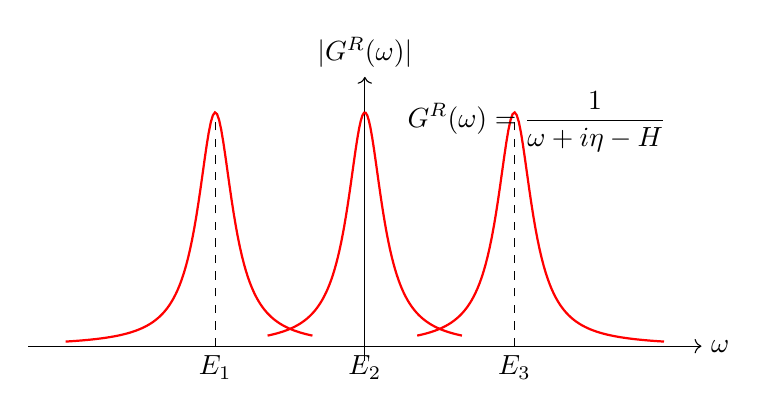
\begin{tikzpicture}[scale=0.95]
\draw[->] (-4.5,0) -- (4.5,0) node[right] {\(\omega\)};
\draw[->] (0,-0.2) -- (0,3.6) node[above] {\(|G^R(\omega)|\)};

\draw[thick,red,domain=-4:-0.7,samples=120] plot (\x,{0.25/((\x+2)^2+0.08)});
\draw[thick,red,domain=-1.3:1.3,samples=120] plot (\x,{0.25/((\x)^2+0.08)});
\draw[thick,red,domain=0.7:4,samples=120] plot (\x,{0.25/((\x-2)^2+0.08)});

\draw[dashed] (-2,0) -- (-2,3.1);
\draw[dashed] (0,0) -- (0,3.1);
\draw[dashed] (2,0) -- (2,3.1);

\node[below] at (-2,0) {\(E_1\)};
\node[below] at (0,0) {\(E_2\)};
\node[below] at (2,0) {\(E_3\)};
\node at (2.3,3.0) {\(\displaystyle G^R(\omega)=\frac{1}{\omega+i\eta-H}\)};
\end{tikzpicture}

\vspace{0.3cm}
The poles of the Green's function correspond to the excitation energies of the system.
\end{frame}

%------------------------------------------------

\begin{frame}{Applying a Green's Function to a Source State}
Let
\[
|b\rangle = \sum_j \beta_j |u_j\rangle.
\]
Then
\[
G(z)|b\rangle
=
\sum_j \frac{\beta_j}{z-E_j}|u_j\rangle.
\]

This has exactly the same structure as
\[
A^{-1}|b\rangle
=
\sum_j \frac{\beta_j}{\lambda_j}|u_j\rangle.
\]

Thus HHL can be interpreted as a quantum Green's-function-style filtering procedure.
\end{frame}

%------------------------------------------------

\begin{frame}{Dynamical Susceptibility}
A standard linear-response object is
\[
\chi(\omega)
=
\langle \psi_0|
\hat{O}^\dagger
\frac{1}{\omega+i\eta-(H-E_0)}
\hat{O}
|\psi_0\rangle.
\]

Defining the source
\[
|b\rangle = \hat{O}|\psi_0\rangle,
\]
we obtain
\[
\chi(\omega)=
\langle b|
\frac{1}{\omega+i\eta-(H-E_0)}
|b\rangle.
\]

Hence HHL is naturally connected to the preparation of response states.
\end{frame}



\begin{frame}{TDHF Equation}
Time-dependent Hartree--Fock is governed by
\[
i \frac{d\rho}{dt} = [h[\rho],\rho].
\]

Linearizing about a stationary solution,
\[
\rho(t)=\rho_0+\delta\rho(t),
\]
yields a linear equation for the fluctuation \(\delta\rho\).
\end{frame}

%------------------------------------------------

\begin{frame}{Linearized TDHF in Frequency Space}
After Fourier transform, one obtains
\[
(\omega I-\mathcal{L})\,\delta\rho(\omega)=s(\omega),
\]
where
\begin{itemize}
\item \(\mathcal{L}\) is the linearized Liouvillian,
\item \(s(\omega)\) is the driving term.
\end{itemize}

This is exactly of the form
\[
Ax=b.
\]
\end{frame}

%------------------------------------------------

\begin{frame}{TDHF as an Inverse-Operator Problem}
The formal solution is
\[
\delta\rho(\omega)=
(\omega I-\mathcal{L})^{-1}s(\omega).
\]

Thus the TDHF response is a resolvent applied to a source term.

This is precisely the same algebraic structure targeted by HHL.
\end{frame}

%------------------------------------------------

\begin{frame}{TDHF / Linear Response Diagram}
\centering
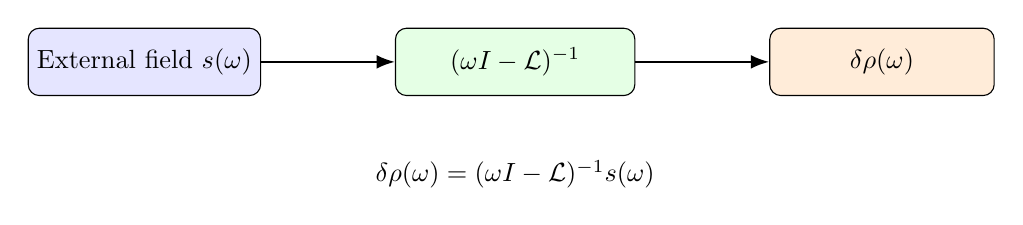
\begin{tikzpicture}[node distance=1.7cm,>=Latex,scale=0.95, every node/.style={scale=0.95}]
\node[draw,rounded corners,fill=blue!10,minimum width=2.8cm,minimum height=0.9cm] (pert) {External field \(s(\omega)\)};
\node[draw,rounded corners,fill=green!10,minimum width=3.2cm,minimum height=0.9cm,right=of pert] (liouv) {\((\omega I-\mathcal{L})^{-1}\)};
\node[draw,rounded corners,fill=orange!15,minimum width=3.0cm,minimum height=0.9cm,right=of liouv] (resp) {\(\delta\rho(\omega)\)};
\draw[->,thick] (pert) -- (liouv);
\draw[->,thick] (liouv) -- (resp);

\node[below=0.7cm of liouv] (text) {\(\delta\rho(\omega)=(\omega I-\mathcal{L})^{-1}s(\omega)\)};
\end{tikzpicture}

\vspace{0.4cm}
The whole linear-response problem is an inverse-operator map from source to response.
\end{frame}

%------------------------------------------------

\begin{frame}{Connection to RPA}
In the small-amplitude limit, TDHF is closely related to the RPA eigenvalue problem
\[
\begin{pmatrix}
A & B \\
-B^* & -A^*
\end{pmatrix}
\begin{pmatrix}
X \\ Y
\end{pmatrix}
=
\omega
\begin{pmatrix}
X \\ Y
\end{pmatrix}.
\]

Equivalently, one can write a driven problem
\[
(\omega I-M)v=s.
\]

Again, the essential structure is resolvent inversion.
\end{frame}


\begin{frame}{Physical Role of QPE in HHL}
From a physics viewpoint:
\begin{itemize}
\item QPE performs a spectral decomposition of the operator,
\item the controlled rotation applies a resolvent-like inverse weight,
\item inverse QPE recombines the filtered eigenmodes.
\end{itemize}

So the logic of HHL is
\[
\text{spectral analysis}
\;\rightarrow\;
\text{inverse weighting}
\;\rightarrow\;
\text{state reconstruction}.
\]
\end{frame}

%------------------------------------------------

\begin{frame}{Unified Conceptual Diagram}
\centering
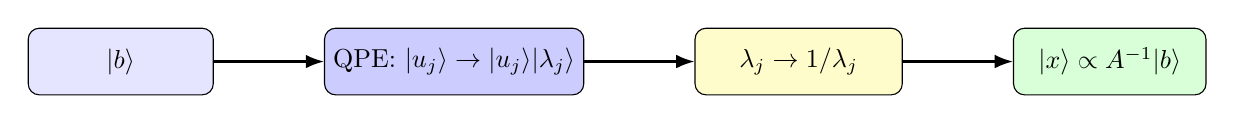
\begin{tikzpicture}[node distance=1.4cm,>=Latex,scale=0.94, every node/.style={scale=0.94}]
\node[draw,rounded corners,fill=blue!10,minimum width=2.5cm,minimum height=0.9cm] (input) {\(|b\rangle\)};
\node[draw,rounded corners,fill=blue!20,minimum width=3.0cm,minimum height=0.9cm,right=of input] (qpe) {QPE: \(|u_j\rangle \to |u_j\rangle|\lambda_j\rangle\)};
\node[draw,rounded corners,fill=yellow!20,minimum width=2.8cm,minimum height=0.9cm,right=of qpe] (filter) {\(\lambda_j \to 1/\lambda_j\)};
\node[draw,rounded corners,fill=green!15,minimum width=2.6cm,minimum height=0.9cm,right=of filter] (output) {\(|x\rangle \propto A^{-1}|b\rangle\)};
\draw[->,thick] (input) -- (qpe);
\draw[->,thick] (qpe) -- (filter);
\draw[->,thick] (filter) -- (output);
\end{tikzpicture}

\vspace{0.5cm}
This is the same logic as in Green's-function and linear-response theory.
\end{frame}


\begin{frame}{Important Caveats}
The conceptual connection is strong, but practical implementation requires:
\begin{itemize}
\item efficient Hamiltonian simulation or block encoding,
\item well-conditioned matrices,
\item efficient state preparation,
\item care with non-Hermitian response matrices.
\end{itemize}

For non-Hermitian problems one often uses a Hermitian embedding such as
\[
\mathcal{H}=
\begin{pmatrix}
0 & M \\
M^\dagger & 0
\end{pmatrix}.
\]
\end{frame}


\begin{frame}{Summary}
\begin{itemize}
\item In the original HHL algorithm, \textbf{QPE is essential}.
\item QPE is the block that resolves the operator spectrally.
\item HHL then implements the spectral filter
\[
\lambda_j \mapsto \frac{1}{\lambda_j}.
\]
\item This makes HHL naturally connected to
\begin{itemize}
\item resolvents,
\item Green's functions,
\item susceptibilities,
\item TDHF and RPA,
\item frequency-domain linear response.
\end{itemize}
\end{itemize}
\end{frame}

%------------------------------------------------

\begin{frame}{Final Conceptual Equivalence}
\[
\boxed{
A^{-1}|b\rangle
\;\sim\;
(zI-H)^{-1}|b\rangle
\;\sim\;
(\omega I-\mathcal{L})^{-1}s
}
\]

\vspace{0.4cm}
\[
\boxed{
\text{HHL}=
\text{QPE}
+
\text{spectral inversion}
+
\text{state reconstruction}
}
\]

HHL is therefore best interpreted as a quantum inverse-operator method.
\end{frame}

\end{document}


\end{document}


